\documentclass[sigconf,anonymous,review]{acmart}

\settopmatter{printacmref=false}
\renewcommand\footnotetextcopyrightpermission[1]{}
\pagestyle{plain}

\acmConference[LaugHSMI '26]{LaugHSMI Workshop at the International Conference on Multimodal Interaction (ICMI)}{October 2026}{Naples, Italy}
\acmYear{2026}
\copyrightyear{2026}

\usepackage{booktabs}

\newcommand{\eg}{e.g.,}
\newcommand{\ie}{i.e.,}

\begin{document}

\title{Does Laughter Fool Deepfake Detectors? Genuine vs.\ Synthetic Laughter in Self-Supervised Speech Representations}

\author{Anonymous Authors}
\affiliation{%
  \institution{Anonymous Institution}
  \city{}
  \country{}
}

\begin{abstract}
As audio generation systems move beyond lexical speech to socially meaningful vocalizations such as laughter, assessing the authenticity of these signals becomes important both for socially intelligent agents and for audio-deepfake detection. We study genuine and synthetic laughter across five synthesis families. Several generators are separable from verified human laughter in WavLM representations---including when the generator is held out of training---but the mismatch is generator-dependent: Bark and Parler-TTS laughter is more continuously voiced and more harmonic than genuine laughter, AudioLDM~2 produces unusually high-pitched and spectrally bright laughter, and reference-conditioned XTTS is acoustically closer but differs in laugh-episode structure. These exploratory results connect synthetic-laughter artifacts to established acoustic correlates of spontaneous versus volitional laughter. We further show that laughter insertion exposes a locality vulnerability in utterance-level deepfake detectors: splicing a socially plausible non-speech region into a fake utterance lets 20\% of fakes evade a detector that otherwise catches 97\% of them, while full-waveform scoring with worst-window aggregation restores robustness (1\% evasion) without retraining, in our controlled setting.
\end{abstract}

\begin{CCSXML}
<ccs2012>
<concept>
<concept_id>10010147.10010178.10010179.10010182</concept_id>
<concept_desc>Computing methodologies~Speech recognition</concept_desc>
<concept_significance>300</concept_significance>
</concept>
<concept>
<concept_id>10003120.10003121.10003122.10003334</concept_id>
<concept_desc>Human-centered computing~User studies</concept_desc>
<concept_significance>100</concept_significance>
</concept>
<concept>
<concept_id>10002978.10003014.10003017</concept_id>
<concept_desc>Security and privacy~Spoofing attacks</concept_desc>
<concept_significance>500</concept_significance>
</concept>
</ccs2012>
\end{CCSXML}

\ccsdesc[500]{Security and privacy~Spoofing attacks}
\ccsdesc[300]{Computing methodologies~Speech recognition}

\keywords{laughter, deepfake detection, speech synthesis, self-supervised representations, non-verbal vocalization, authenticity}

\maketitle

\section{Introduction}
Laughter is among the most socially consequential non-verbal vocalizations: it signals affiliation, regulates conversation, and is produced and perceived along a spontaneous--volitional continuum with distinct acoustic correlates \cite{scott2014social,bachorowski2001acoustic,bryant2014animal,lavan2016laugh}. Modern generative audio systems now produce laughter on demand. Token-based text-to-speech (TTS) systems such as Bark emit \texttt{[laughter]} events \cite{bark2023}; description-conditioned TTS such as Parler-TTS can be prompted to laugh \cite{lyth2024parler}; diffusion text-to-audio models such as AudioLDM~2 generate free-form laughter \cite{liu2024audioldm2}; and zero-shot voice-cloning TTS such as XTTS can imitate a reference laugh \cite{casanova2024xtts}. If synthetic laughter becomes socially convincing, it matters twice over: socially intelligent agents will need to assess the authenticity of laughter they hear, and audio-deepfake detectors---built and evaluated almost exclusively on read or conversational \emph{speech} \cite{wang2020asvspoof,muller2022does}---will encounter non-speech vocalizations they were never trained to judge.

This paper asks two questions at that intersection. \emph{First}, how does synthetic laughter differ acoustically and representationally from genuine laughter, and are the differences uniform across synthesis families? \emph{Second}, what happens when laughter is inserted into the input of a state-of-the-art utterance-level deepfake detector?

We make three contributions. \textbf{(1) A generator-family taxonomy of synthetic laughter} (Sec.~\ref{sec:taxonomy}): in an exploratory analysis grounded in established acoustic correlates of spontaneous versus volitional laughter, speech-derived generators (Bark, Parler-TTS) produce laughter that is too continuously voiced and too harmonic; AudioLDM~2 approximates genuine voicing structure but is abnormally high-pitched and spectrally bright; and reference-conditioned XTTS is acoustically closest yet differs in laugh-episode topology. \textbf{(2) Evidence that self-supervised speech representations carry generator-dependent laughter-authenticity signal} (Sec.~\ref{sec:ssl}): after controlling clip length, silence, and loudness, WavLM embeddings separate genuine from synthetic laughter well above a content-free acoustic baseline for four of five generator families, and the signal partially transfers to held-out generators---though the best layer depends on the generator. \textbf{(3) A controlled detector-robustness finding with a training-free mitigation} (Sec.~\ref{sec:insertion}): inserting a short laughter segment into a spoofed utterance shifts a strong detector's score so that 20\% of previously caught fakes evade detection; causal masking controls attribute the shift to the inserted region, and full-waveform scoring with worst-window aggregation reduces evasion to 1\% without retraining.

\section{Related work}
\textbf{Genuine vs.\ volitional laughter.} Human laughter is acoustically heterogeneous, spanning voiced song-like bouts and unvoiced grunt- or snort-like calls \cite{bachorowski2001acoustic,provine1991laughter}. Spontaneous laughter differs systematically from volitional (posed) laughter: it is less like speech in its production, with higher pitch, greater unvoiced proportion, and reduced articulatory shaping \cite{bryant2014animal,lavan2016laugh,ruch2001expressive}. We use these findings as reference axes for characterizing \emph{synthetic} laughter, which can be viewed as an extreme point on the volitional side: laughter produced by a system trained mostly on speech.

\textbf{Laughter corpora and detection.} Laughter resources include acted and induced corpora such as MAHNOB \cite{petridis2013mahnob} and crowd-sourced vocalization sets such as VocalSound \cite{gong2022vocalsound}; robust laughter detectors exist for conversational audio \cite{gillick2021laughter}. Laughter \emph{synthesis} has been studied as a goal in itself \cite{mori2019laughter}, but the authenticity of laughter produced by modern general-purpose generators has received little attention.

\textbf{Audio deepfake detection.} Current detectors couple self-supervised front-ends with graph-attention back-ends \cite{tak2022automatic,jung2022aasist} and are trained on speech-only corpora such as ASVspoof~2019 \cite{wang2020asvspoof}; generalization beyond the training domain is a known weakness \cite{muller2022does}. Closest to our third contribution, PartialSpoof \cite{zhang2023partialspoof} shows that short fake segments embedded in genuine utterances challenge utterance-level countermeasures. We study the \emph{converse} insertion---a genuine-sounding non-speech segment embedded in a fake utterance---and show it, too, exploits utterance-level score aggregation. Emotion-targeted deepfakes \cite{zhao2022emofake} are precedent for generation moving beyond neutral read speech; laughter extends this to non-lexical vocalization.

\section{Data and methods}
\label{sec:methods}

\textbf{Genuine laughter.} We use laughter clips from VocalSound \cite{gong2022vocalsound}, a crowd-sourced corpus of non-speech vocalizations from over 3{,}000 speakers, as the verified-human anchor. For the acoustic analyses we manually verified a subset containing at least 2\,s of active laughter.

\textbf{Synthetic laughter (five families, 232 clips).} We generate laughter with four open engines spanning distinct synthesis paradigms: \emph{Bark} \cite{bark2023} laughter-only \texttt{[laughter]} tokens (100 clips) and inline \texttt{[laughs]} within speech (40); \emph{Parler-TTS} \cite{lyth2024parler} description-conditioned laughter (32); \emph{AudioLDM~2} \cite{liu2024audioldm2} text-to-audio laughter from prompts such as ``hearty human laughter'' (30); and \emph{XTTS-v2} \cite{casanova2024xtts} laughter cloned from VocalSound reference clips (30). Bark and Parler-TTS are speech-LM-derived; AudioLDM~2 is a general audio diffusion model; XTTS is reference-conditioned.

\textbf{Confound control.} Corpus-level nuisance variables (clip duration, silence padding, loudness, channel) can separate any two corpora. All representational probes therefore operate on energy-trimmed, fixed 2\,s active segments, peak-normalized, with groups balanced (N=30/group within-generator; N=20/group for held-out-generator runs). As a floor, we train the identical probe on an 8-scalar \emph{content-free} feature set (duration, lead/trail silence, RMS, spectral centroid/rolloff, zero-crossing rate, high-frequency energy): any WavLM advantage over this floor cannot be explained by those recording-level covariates. Label-shuffle (AUC 0.48) and real-vs-real split (0.45) controls are at chance.

\textbf{Representational probes.} We extract WavLM-Large \cite{chen2022wavlm} hidden states and train logistic-regression probes on mean-pooled segment embeddings (with PCA-20) to separate genuine from synthetic laughter: (i) \emph{within-generator}, 5-fold cross-validated per family, against the content-free floor; (ii) \emph{held-out-generator}, training on genuine laughter plus four families and testing on the fifth and unseen genuine clips (50 resamples), at layers 0, 3, and 12.

\textbf{Acoustic descriptors.} For the taxonomy we compute literature-aligned full-bout descriptors: voiced fraction, voiced-burst and unvoiced-run durations, voicing transition rate, an autocorrelation harmonicity proxy, F0 statistics, spectral center of gravity, bout duration, and inter-onset interval variability \cite{bachorowski2001acoustic,lavan2016laugh}. Group differences are reported as Cliff's~$\delta$ with Mann--Whitney $p$-values, uncorrected---this analysis is exploratory (N=20/group).

\textbf{Detector and insertion protocol.} The detector is an utterance-level countermeasure representative of the current SSL+graph-attention recipe \cite{tak2022automatic,jung2022aasist}: a WavLM front-end, BiLSTM, and graph-attention \cite{velickovic2018graph} pooling head, trained on ASVspoof~2019~LA \cite{wang2020asvspoof}; it scores a 3\,s center crop and reaches 5.33\% EER on a balanced 150+150 evaluation set (in-domain). Into a random 70\% of the spoofed files (n=105) we splice one Bark laughter clip at a random position (start/mid/end); paired file IDs allow per-file before/after comparison. Controls: \emph{unmask} (splice the inserted region back out --- tests for seam/crop artifacts), \emph{silence} (zero the region, keep the timeline), \emph{real laughter} (VocalSound inserts, same protocol), and \emph{real speech} (LibriSpeech \cite{panayotov2015librispeech} inserts, level-matched). The \emph{mitigation} slides 3\,s windows over the full waveform and aggregates window scores by mean, 90th percentile, or max (worst window).

\begin{figure}[t]
  \centering
  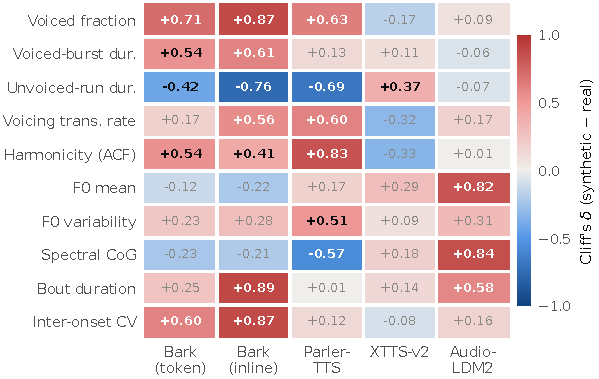
\includegraphics[width=\columnwidth]{figs/fig_taxonomy.pdf}
  \caption{Generator-family acoustic taxonomy of synthetic laughter. Cells show Cliff's~$\delta$ (synthetic $-$ genuine) for literature-aligned laughter descriptors vs.\ the verified real anchor (N=20/group); bold marks uncorrected $p<.05$. Speech-derived Bark/Parler are over-voiced and over-harmonic; AudioLDM~2 matches voicing structure but is high-pitched and bright; XTTS deviates mainly in episode structure (longer unvoiced runs).}
  \label{fig:taxonomy}
  \Description{Heatmap of Cliff's delta values for ten acoustic features across five laughter generators, showing distinct per-generator signatures.}
\end{figure}

\section{Results}

\subsection{A generator-family taxonomy of synthetic laughter}
\label{sec:taxonomy}
Figure~\ref{fig:taxonomy} summarizes the exploratory acoustic comparison of each synthesis family against verified genuine laughter. Three profiles emerge.

\textbf{Speech-derived TTS is over-voiced and over-harmonic.} Genuine laughter in our anchor is predominantly unvoiced (voiced fraction 0.24) with long unvoiced runs (0.93\,s) and low harmonicity ($-2.1$\,dB) --- consistent with the classic finding that spontaneous laughter contains a large proportion of unvoiced, noisy calls \cite{bachorowski2001acoustic,lavan2016laugh}. Bark and Parler-TTS laughter inverts this profile: voiced fraction 0.52--0.62 ($\delta$ up to $+0.87$), unvoiced runs of only 0.28--0.67\,s, and positive harmonicity ($+0.7$ to $+4.0$\,dB). Systems whose training distribution is dominated by speech appear to produce laughter the way people produce \emph{volitional} laughter: by speaking it.

\textbf{AudioLDM~2 fails on register, not voicing.} The diffusion audio model approximates the genuine voiced/unvoiced organization (voiced fraction 0.235 vs.\ 0.239) but is far higher-pitched (mean F0 432 vs.\ 244\,Hz, $\delta=+0.82$) and spectrally brighter (center of gravity 2598 vs.\ 1916\,Hz, $\delta=+0.84$) --- an exaggerated, caricature-like laugh texture.

\textbf{XTTS is acoustically closest but differs in episode topology.} Reference-conditioned XTTS matches the anchor on most descriptors, with its largest deviations in laugh-episode structure: longer unvoiced runs (1.76 vs.\ 0.93\,s, $p=.048$) and fewer voicing transitions (1.10 vs.\ 1.72/s), suggesting separated, unit-like laughs rather than the denser alternation of calls and gaps in genuine bouts. Because its references come from the same corpus as the real anchor, source leakage may deflate its differences (Sec.~\ref{sec:limitations}).

The heterogeneity is itself the finding: generators miss \emph{different} parts of the genuine laughter-production repertoire, so no single ``synthetic laughter'' prototype exists to detect.

\begin{figure}[t]
  \centering
  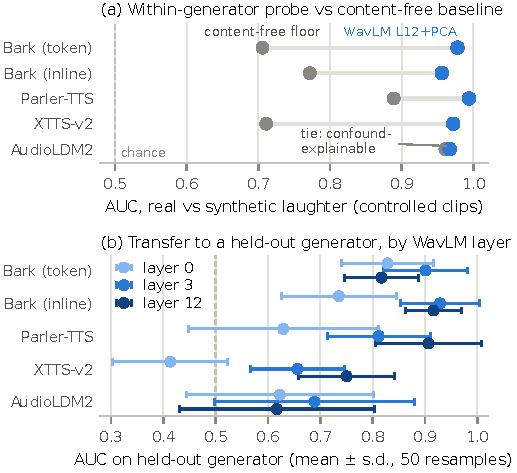
\includegraphics[width=\columnwidth]{figs/fig_separability.pdf}
  \caption{Genuine vs.\ synthetic laughter in WavLM. (a) On length-, silence-, and loudness-equalized clips, WavLM probes exceed a content-free acoustic floor for four of five families; the AudioLDM~2 tie means its separation is confound-explainable. (b) Probes trained on four families partially transfer to the held-out fifth; the best layer is generator-dependent.}
  \label{fig:separability}
  \Description{Dumbbell chart of AUC versus a content-free baseline for five generators, and dot plot with error bars showing transfer AUC to held-out generators for WavLM layers 0, 3 and 12.}
\end{figure}

\subsection{Laughter authenticity in self-supervised representations}
\label{sec:ssl}
Figure~\ref{fig:separability}a shows the confound-controlled within-generator probes. WavLM layer-12 probes separate genuine from synthetic laughter at AUC 0.956--0.994 for Bark (token and inline), Parler-TTS, and XTTS, exceeding the content-free floor by $+0.11$ to $+0.27$. This margin cannot be attributed to duration, silence, or loudness, so the embeddings carry laughter-specific authenticity signal for these families. AudioLDM~2 is the exception: its WavLM AUC (0.967) ties the floor (0.961), so we make no representational claim for it --- notable because it is also the family whose voicing structure best matches genuine laughter (Sec.~\ref{sec:taxonomy}).

Figure~\ref{fig:separability}b applies the stricter held-out-generator protocol. A probe trained on genuine laughter plus four families still detects the unseen fifth well above chance for the speech-derived families (layer 3: Bark-inline 0.93, Bark-token 0.90, Parler 0.81; layer 12: Parler 0.91), moderately for XTTS (layer 12: 0.75), and unreliably for AudioLDM~2 ($0.69\pm0.19$). The layer that transfers best changes with the generator --- early layers for Bark, deeper ones for Parler and XTTS --- so the transferable signature is generator- and layer-dependent rather than a single universal ``synthetic laughter'' direction, mirroring the acoustic taxonomy.

\subsection{Laughter insertion and detector locality}
\label{sec:insertion}
Figure~\ref{fig:insertion} presents the detector study. Splicing one Bark laughter clip into each fake drops the mean spoof score from 0.899 to 0.604 (paired Wilcoxon $p<10^{-6}$, rank-biserial $r=-0.78$); at the clean-EER operating point the detector's catch rate on these fakes falls from 97\% to 80\%, \ie\ \textbf{20\% of augmented fakes evade} a detector that is otherwise strong in-domain. The masking controls establish locality: removing the inserted region restores the original score (0.891), so the effect is the region itself, not a splice artifact; silencing the region drops scores even further (0.363).

Crucially, the vulnerability is \emph{not laughter-specific}. Real VocalSound laughter also evades, though less strongly ($\Delta=-0.13$); a level-matched real \emph{speech} insert drops the score as much as synthetic laughter does ($-0.31$ vs.\ $-0.29$); and the effect does not grow with the fraction of the scored crop occupied by laughter (Spearman $\rho\approx0$). The picture is of \emph{pooling dilution}: the detector aggregates frame-level evidence over a single 3\,s crop, so any locally non-spoof-like region dilutes the utterance score. Laughter is an evasion vector \emph{of opportunity} --- unlike a stranger's sentence, an inserted laugh is socially plausible and unlikely to arouse suspicion in a conversational deepfake.

This diagnosis directly implies a training-free mitigation (Fig.~\ref{fig:insertion}b): score \emph{all} 3\,s windows of the waveform and let the most spoof-like window decide. Sliding windows alone (mean aggregation) cut evasion from 20\% to 2.9\% by ensuring the synthetic material cannot fall outside the scored crop; worst-window (max) aggregation removes the dilution channel and reduces evasion to \textbf{1.0\%}, raising catch rate on augmented fakes to 99\% at a modest clean-EER cost (5.33\%$\to$4.33\%). Local scoring, not retraining, closes the blind spot in this controlled setting.

\begin{figure*}[t]
  \centering
  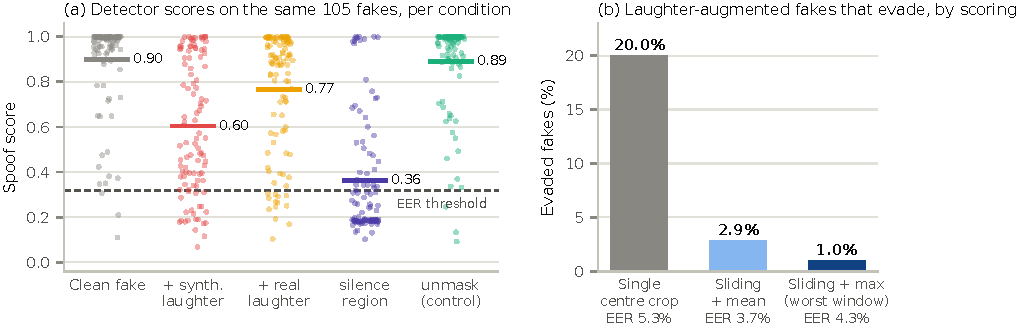
\includegraphics[width=\textwidth]{figs/fig_insertion.pdf}
  \caption{Laughter insertion exposes a locality vulnerability, and local scoring repairs it. (a) Spoof scores of the same 105 ASVspoof2019-LA fakes under each condition (horizontal bar = mean; dashed line = clean-EER threshold): synthetic and real laughter inserts pull fakes toward the genuine side; removing the inserted region (unmask) restores the original score. (b) Fraction of laughter-augmented fakes that evade detection under three scoring schemes.}
  \label{fig:insertion}
  \Description{Left: strip plot of detector spoof scores for five conditions showing score drops after laughter insertion. Right: bar chart showing evasion falling from 20 percent with single-crop scoring to 1 percent with worst-window scoring.}
\end{figure*}

\section{Discussion}
Our findings link generative-model artifacts to the psychology of laughter production. The spontaneous--volitional literature holds that genuine laughter departs from speech-like phonation: more unvoiced material, less harmonic structure, higher and more variable pitch produced by an ``unspeechlike'' vocal act \cite{bachorowski2001acoustic,bryant2014animal,lavan2016laugh}. Speech-trained generators fail exactly along this axis --- they \emph{speak} their laughter, producing the over-voiced, over-harmonic profile of volitional laughter. A general-audio model (AudioLDM~2) escapes that failure mode but overshoots register; a reference-cloning model (XTTS) inherits genuine acoustics from its reference yet reassembles them with different episode timing. For socially intelligent agents, this suggests authenticity assessment should be multi-axis (voicing structure, register, episode topology) rather than a single genuine-vs-synthetic score; for generation, each family has a distinct, nameable gap to close.

For deepfake detection, the two halves of the paper meet in a design implication. Laughter regions carry usable authenticity signal in SSL representations (Sec.~\ref{sec:ssl}), yet the utterance-level detector does not exploit it --- worse, inserted laughter \emph{dilutes} its decision (Sec.~\ref{sec:insertion}). Detectors that score local windows and reason about non-speech regions explicitly could both resist insertion attacks and use synthetic-laughter artifacts as evidence. Our worst-window result shows the first half of that agenda needs no new training; complementarily, PartialSpoof-style localization \cite{zhang2023partialspoof} addresses the same aggregation weakness from the training side.

\section{Limitations and ethics}
\label{sec:limitations}
\textbf{Single real anchor.} All genuine laughter comes from VocalSound; despite our content-free floor and controls for length, silence, and loudness, residual corpus or channel characteristics may contribute to separability, and the acoustic profile of the anchor (crowd-sourced, prompted laughter) may not represent fully spontaneous conversational laughter. Replication with a second, independently recorded laughter corpus is the immediate next step. \textbf{XTTS source leakage.} XTTS clips are cloned from VocalSound references, which may transfer channel or speaker characteristics into the synthetic set and deflate its measured differences. \textbf{Exploratory statistics.} Acoustic comparisons use N=20/group with uncorrected per-generator tests, and the harmonicity measure is an autocorrelation proxy rather than a standard HNR; the taxonomy is a characterization to be confirmed, not a confirmed mechanism. \textbf{Single detector and dataset.} The insertion study uses one (representative) detector architecture on ASVspoof~2019~LA; the magnitude of insertion effects may differ across architectures and corpora, and our mitigation is evaluated against the specific insertion attack studied here, not against an adaptive adversary.

\textbf{Ethics.} This work characterizes an evasion vector; we judge disclosure appropriate because the insertion attack is simple enough to be discovered independently, while the mitigation we provide is immediately deployable without retraining. Synthetic laughter itself raises ethical questions beyond fraud: laughter signals affiliation and empathy, and agents that deploy convincing fake laughter may manipulate social trust. Datasets, generation scripts, and analysis code will be released to support replication.

\begin{acks}
Omitted for double-blind review.
\end{acks}

\bibliographystyle{ACM-Reference-Format}
\bibliography{references}

\end{document}
